% file: main.tex
\documentclass[10pt,oneside]{journal}
\usepackage{mathtools}
\usepackage{fullpage}
\usepackage{listings}
\usepackage{color}
\usepackage{float}
\usepackage{graphicx}
\usepackage[space]{grffile}
 
\definecolor{dkgreen}{rgb}{0,0.6,0}
\definecolor{gray}{rgb}{0.5,0.5,0.5}
\definecolor{mauve}{rgb}{0.58,0,0.82}
\definecolor{dkred}{rgb}{0.7,0,0}




\lstset{ %
  language=Python,                % the language of the code
  basicstyle=\small,              % the size of the fonts that are used for the code
  numbers=left,                   % where to put the line-numbers
  numberstyle=\small\color{gray},  % the style that is used for the line-numbers
  stepnumber=1,                   % the step between two line-numbers. If it's 1, each line 
                                  % will be numbered
  numbersep=5pt,                  % how far the line-numbers are from the code
  backgroundcolor=\color{white},      % choose the background color. You must add \usepackage{color}
  showspaces=false,               % show spaces adding particular underscores
  showstringspaces=false,         % underline spaces within strings
  showtabs=false,                 % show tabs within strings adding particular underscores
  frame=single,                   % adds a frame around the code
  rulecolor=\color{black},        % if not set, the frame-color may be changed on line-breaks within not-black text (e.g. commens (green here))
  tabsize=4,                      % sets default tabsize to 2 spaces
  captionpos=b,                   % sets the caption-position to bottom
  breaklines=true,                % sets automatic line breaking
  breakatwhitespace=false,        % sets if automatic breaks should only happen at whitespace
  title=\lstname,                   % show the filename of files included with \lstinputlisting;
                                  % also try caption instead of title
  keywordstyle=\color{blue},          % keyword style
  commentstyle=\color{dkgreen},       % comment style
  stringstyle=\color{mauve},         % string literal style
  escapeinside={\%*}{*)},            % if you want to add a comment within your code
  morekeywords={class,private,procedure,device},               % if you want to add more keywords to the set
  emphstyle=\color{dkred},
  emph={MPI_BCAST,MPI_INTEGER,MPI_COMM_WORLD,ierror,MPI_RECV,MPI_SEND,MPI_DOUBLE_PRECISION,MPI_SCATTER,MPI_GATHER,MPI_INIT,MPI_COMM_SIZE,MPI_COMM_RANK,MPI_WTIME,MPI_BARRIER}
}

\begin{document}
	
	%!TEX root = ../main.tex
% file: title.tex
\begin{center}
\textsc{\Large MCS507 Project Two:\\}
\textsc{Study a Mathematical Software Package: Earth}
\end{center}
\begin{minipage}{0.6\textwidth}
\begin{flushleft}
	Prepared By: Adam McElhinney
\end{flushleft}
\end{minipage}
\begin{minipage}{0.39\textwidth}
\begin{flushright}
	October 28, 2012
\end{flushright}
\end{minipage}\\[0.01in]
\hrule
	
    %!TEX root = ../main.tex
% file: assignment2.tex


\graphicspath{{C:/Documents and Settings/amcelhinney/My Documents/GitHub/MCS507ProjectTwo/tex/include/}}

\section{Assignment One: Overview and Illustrative Example.} % (fold)
\label{sec: Main Problem}
Our first objective is to identify the main problem this software aims to solve. We then provide an overview of the software package and the algorithms used. We conclude with an illustrative example that displays the utility of this software.

\subsection{Main Problem this Software Aims to Solve} % (fold)
\label{sub:methoda}
The Earth software package is an implementation of the Multivariate Adaptive Regression Splines (MARS) technique developed by Jerome H. Friedman of Stanford University. Interestingly, the reference MARS is copywritten, thus open source implementations of the software are referred to as Earth. The purpose of this technique is similar to that of all regression techniques, namely to fit a function to a set of data. However, the Earth software specifically seeks to do this in a manner that has the following advantages:
\begin{enumerate}
\item Ability to easily handle non-linear data sets
\item Ease of interpretation 
\item Ability to handle large datasets
\item Automatic variable selection
\end{enumerate}


% subsection Main Problem this Software Aims to Solve (end)

\subsection{Overview of the Software and Algorithms} % (fold)
The Earth software package relies on the application of splines to construct the function to predict the target variable. Broadly speaking, a “spline” is simply a function constructed in various segments from other polynomial functions. The MARS technique relies on a type of splines known as hinge functions, which can be represented in the form:  

\begin{equation}
h_{j}=\max (0,x-c)
\end{equation}

The constant c is referred to as the knot. The Earth software then uses these functions to divide the data into mutually exclusive segments and then fit a model to each individual function. This is done in such a manner as to minimize some objective function. One commonly used objective function is the residual sum of squares (RSS).

\begin{equation}
RSS=\sum_{i=1}^{n} (y_{i}-f(x_{i}))^{2}
\end{equation}

To illustrate, let us consider the typical regression equation where we seek to build a model that predicts the value of the $y_{i}$-th obvseration based on some values of $x$.

\begin{equation}
y_{i}=\beta _{0}+\sum_{i=1}^{M}\beta _{i}*x_{i}
\end{equation}

The Earth software then modifies this model to have the following form (where $h_{i}$ represents the hinge function in equation 1).

\begin{equation}
y_{i}=\beta _{0}+\sum_{i=1}^{M}\beta _{i}*h_{i}(x_{i})
\end{equation}

To fit this model, the Earth software relies on two distinct steps.
\begin{enumerate}


\item Forward Pass: In this step, the model starts with just one intercept term composed of the mean of the target (y) variables. Then the software divides the data into two distinct sets via a pair of basis functions. The area dividing point between these two areas is the knot referred to in equation 1. The position of this knot is calcuated such that it results in the maximum reduction in the $RSS$ in equation 2. This process is repeated until the software has reached a maximum number of terms (as defined by the user prior to initializing the model), or until the change in $RSS$ is too small to continue.

\item Backward Pass: The result of the first step will be a model that fits the data set extremely closely, however it is likely that the model will generalize well to other data. Thus, the backward pass (sometimes referred to as pruning) is applied. In this step, the model searches for the basis functions that contribute to the smallest increase in the goodness of fit. However, the $RSS$ will always favor a model with more parameters, so a goodness of fit measure that penalizes additional parameters is needed. This is referred to as the Generalized Cross Validation $GCV$.



\begin{equation}
GCV=\frac{\sum_{i=1}^{n} (y_{i}-f(x_{i}))^{2}}{1-\frac{C}{n}}
\end{equation}

where $C=1+c*d$, $n$ is the number of observations in the data, $d$ is the number of independent basis functions and $c$ is a penality for adding a basis function.
 
\end{enumerate}


% subsection Overview of the Software and Algorithms (end)


\subsection{Illustrative Example of the Earth Software} % (fold)

To illustrate usage of the Earth software, a simple example data set was generated using the Data Painter tool from the Orange Machine Learning Python library. This data set is composed of an $x$ variable which we attempt to use to predict the value of the $y$ variable. We begin by loading the data, verifying the column names, and then inspect the data.

\begin{lstlisting}[caption={Load and Inspect the Data},label=lst:expected_times,firstnumber=15]

  # Remember to add the "class" keyword to the third line, under the target variable. See here:
  # http://orange.biolab.si/doc/tutorial/load-data/
  data = orange.ExampleTable("painted_data_wo_outlier")
  print data.domain.attributes
  print data[:4]
\end{lstlisting}

After reviewing the data, we convert it to \emph{Numpy} arrays and plot the data using \emph{Matplotlib}.

\begin{lstlisting}[caption={Convert to Array and Plot},label=2nd,firstnumber=21]
X, Y = data.to_numpy("A/C")

pl.plot(X, Y, ".r")
pl.title('Example Data Set')
pl.show()

\end{lstlisting}



\begin{figure}[H]
    \centering
       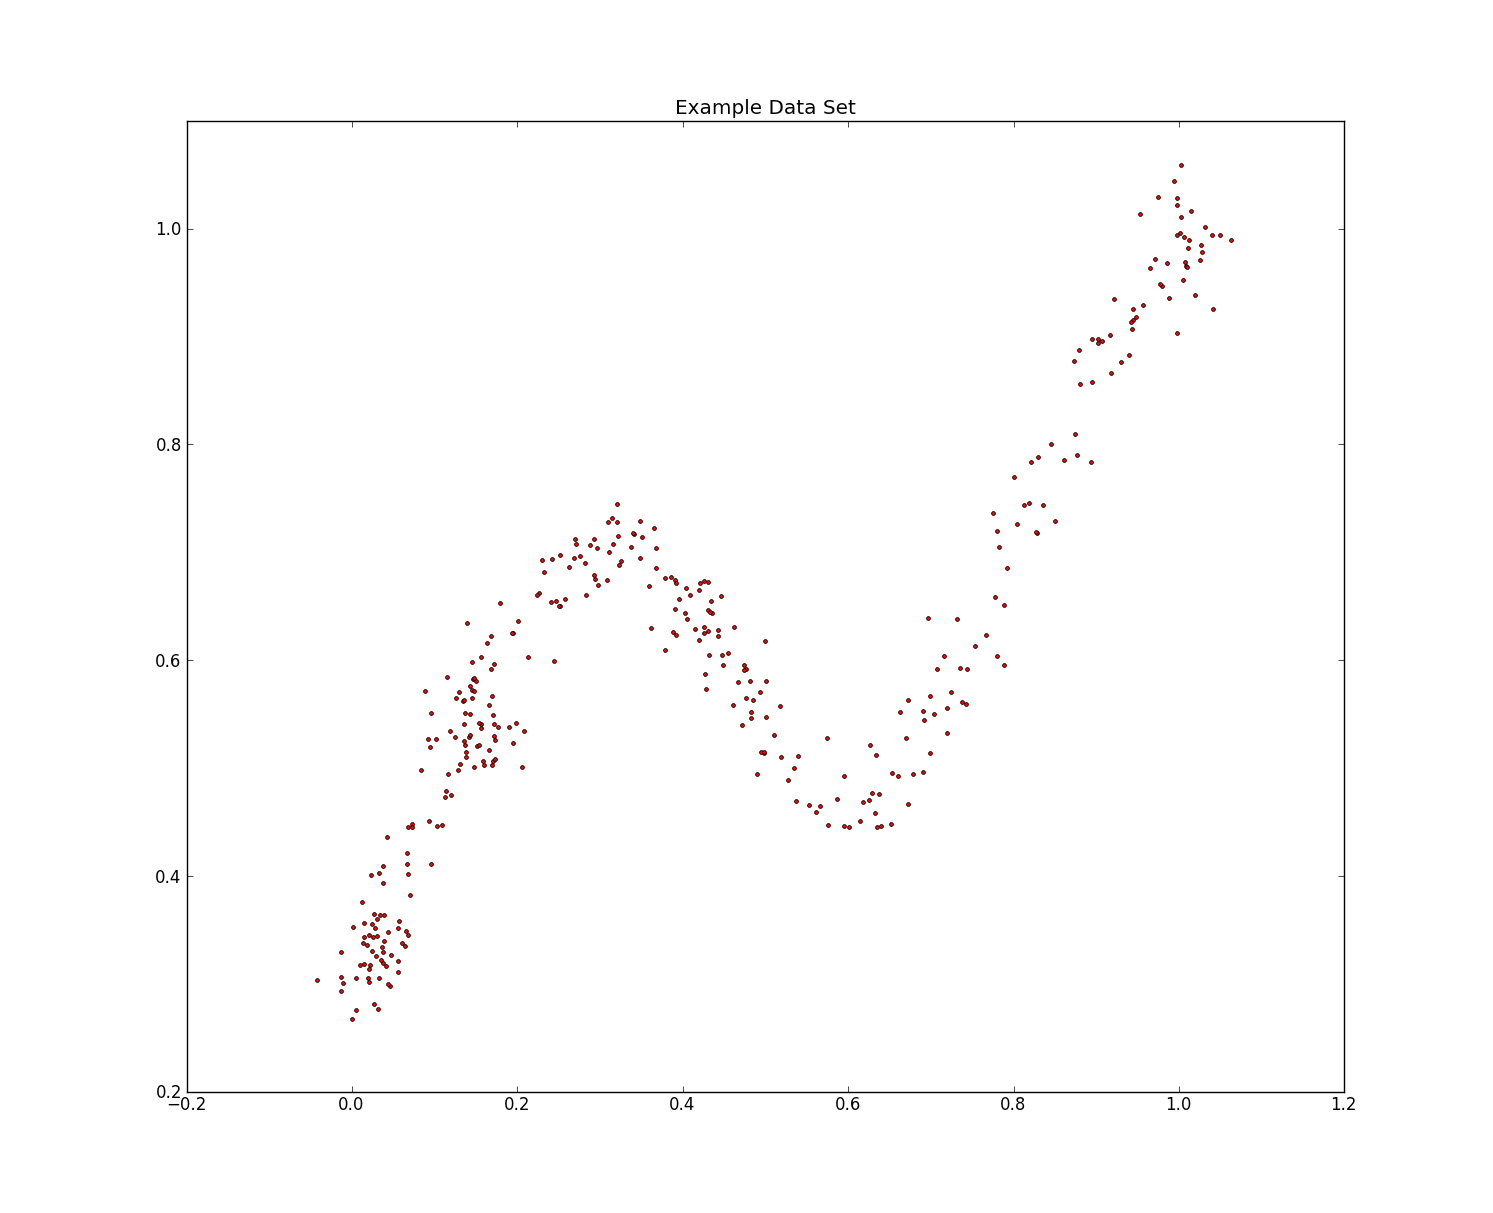
\includegraphics[width=6.5in]{example_data.png}
    \caption{Example Data}
    \label{Example Data}
\end{figure}

As can be seen from the graph, the data exhibits an irregular shape and the density of the points varies as one moves along the x-axis. Thus, this example should prove interesting to test to utility of the Earth software. Next, we use Earth to fit the data and examine the model. 

\begin{lstlisting}[caption={Fit the Data},label=3rd,firstnumber=27]
earth_predictor = earth.EarthLearner(data)
print earth_predictor

\end{lstlisting}

\begin{equation}
	Y =   1.486   +1.445 * \max (0, X - 0.744)   -1.590 * \max (0, 0.744 - X)   -1.818 * \max (0, X - 0.244)
\end{equation}
\begin{equation}
\nonumber
	+2.625 * \max (0, X - 0.640)   -0.682 * \max (0, X - 0.404)   -1.661 * \max (0, X - 0.979)
\end{equation}


Next, we would like to see how well this model predicts the data. One strategy is to plot the values the Earth model predicts and compare them with the actual data. This is done by creating a \emph{Numpy} array of $x$-values and then using the Earth model to predict the values of $y$.

\begin{lstlisting}[caption={Compare the Predicted vs Actual Values and Plot the Results},label=2nd,firstnumber=29]
earth_predictor = earth.EarthLearner(data)
print earth_predictor
linspace = numpy.linspace(min(X), max(X), 20)
predictions = [earth_predictor([s, "?"]) for s in linspace]
pl.plot(X, Y, ".r")
pl.plot(linspace, predictions, "-b")
pl.title('Example Data Set with Line Fit by MARS')
pl.show()
\end{lstlisting}

\begin{figure}[H]
    \centering
       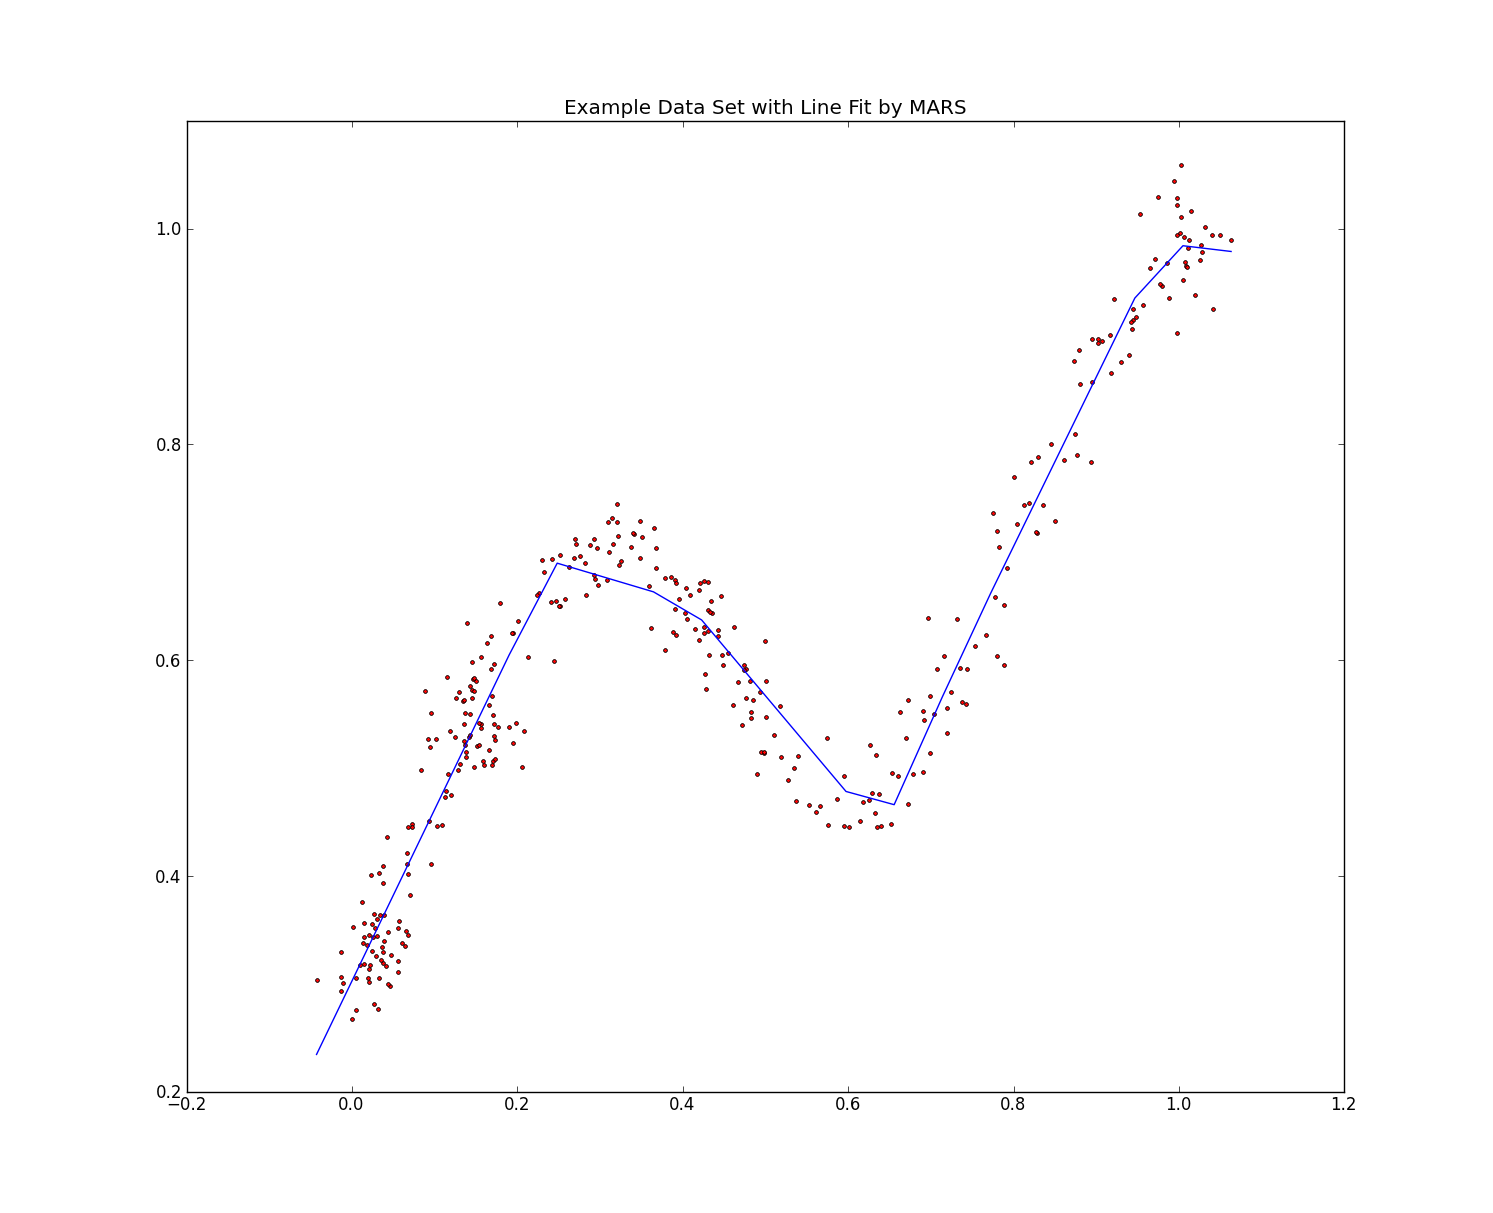
\includegraphics[width=6.5in]{example_data_fit.png}
    \caption{Example Data Set with Line Fit by MARS}
    \label{Example Data}
\end{figure}

Figure 2 shows us that the model output by the Earth software fits the data quite well. It appears that the knots are located close to the inflection points in the data.






% section section_name (end)

	

	
	
\end{document}